\section{MSE Assessors}

Assessors were conceived as specialized data processing modules able
to assess, filter and transform individual data into a cohesive,
synoptic assessment of hydrological states used as decision
variables. Recent development has resulted in two implementations of
Assessors: the WCU Assessor, and the WMM Assessor. As a matter of
convenience, these implementations are hybrid Assessor/Supervisor
constructs, they directly control water flows at simulated hydraulic
structures.

The primary function of the MSE Assessors is to estimate the
interbasin management flows which are compatible with the hydrologic
model state response over periods of 1 day, and which satisfy
operational constraints and objectives.  On a regional scale, the
problem is congruent with many historical applications of optimization
techniques aimed at estimating water resource allocations in a
multibasin network flow problem. In the context of the SFRSM this
would include special operations for regional water supply or CERP
projects. 

\subsection{Operational Problem Statement}

Consider a collection of managed basins with controlled flow conduits
between basins. For example, Figure \ref{fig:connectedBasins}
represents a water control network with basins B1 through B6 where
$q_{12}$ indicates the flow from basin B1 to basin B2.

\begin{figure}
 \begin{center}
  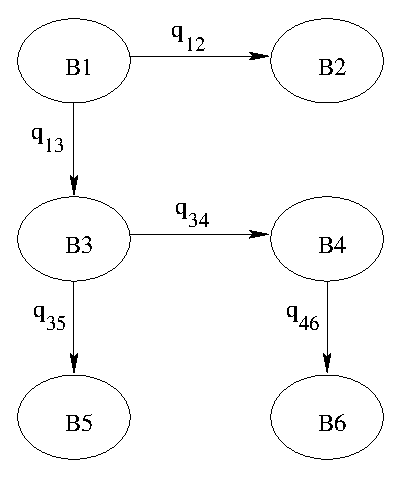
\includegraphics[scale=.75]{Graphics/connectedBasins.eps}
 \end{center}
 \caption{\label{fig:connectedBasins} Water control network of connected basins.}
\end{figure}

In the context of the RSM, a basin consists of a set of:
\begin{itemize}
 \item aquifer/land surface mesh cells, and a collection of canal
   segments or other waterbodies such as lakes, within the confines of
   the basin cells, or
 \item simple basin or lake water body.
\end{itemize}

To facilitate representation of a basin network as a single, managed
water resource, the abstraction Water Control Unit (WCU) refers to the
collection of canal segments within the basin, or the simple basin or
lake waterbody. Each WCU has associated with it a set of operational
constraints. For example a maintenance level specifies a water level
minimum target value for water supply or environmental purposes, while
a flood control level indicates a WCU maximum water level target
value. The flow conduits between basins represent controlled hydraulic
structures. The $q$ values are actually flows between WCU's through a
structure. Each structure may have operational constraints such as a
maximum flow capacity, or maximum/minimum flow values dictated by
water supply or environmental objectives. Functionally, the flow
between two basins depends on both hydrological state information ($s$),
and a managerial control value ($\chi$). The control value is itself a
function of $s$, as well as a function of operational constraints and
objectives ($\lambda$). This can be expressed as:

\begin{align}\label{eqn:interbasinFlow}
 q = f(s,\chi(s,\lambda))
\end{align}

As described in a later section, the state information constitutes
observations of a nonlinear dynamic system.

The flows in Figure \ref{eqn:interbasinFlow} are instantaneous values
which vary continuously, and which we assume are differentiable as
many times as needed. In the context of an RSM implementation used as
a water resource management evaluation or planning tool, the flow
metric of interest is typically a cumulative flow over a period of
time which meets the management objectives. Accordingly, we define the
cumulative flow from basin $n$ to basin $m$ over the time period starting
at $t_s$ and ending at $t_e$ as:

\begin{align}\label{eqn:CumBasintoBasin}
  Q^{se}_{nm} = \int_{t_s}^{t_e}q_{nm}(t)dt
\end{align}

Specifically, in the RSM application to the south Florida region, a
daily timestep has been specified as the simulation increment, i.e.,
$\Delta t = t_e - t_s = 1$ day. This constraint is consistent with a large body
of existing simulation results and database of historical structure
flows and water levels. Further, the model period of record can span
30 years or more, and the large timestep is desirable to limit
simulation run times. However, even at small timesteps on the order of
minutes, the same theory applies. We will denote the cumulative
interbasin flow over a daily time period as $Q_{nm}$. Estimation of the
cumulative flows $Q_{nm}$ over a simulation timestep of 1 day is the
primary objective of the WMM Assessor (Section 2.4), and of the linear
programming models which are under development (Sections 2.7 and 2.8).

\subsection{RSM State Estimation}

RSM is a state estimator. We denote estimates of variables with
italics. RSM allows independent abstraction of hydrological and
managerial state variables through the interoperation of the
Hydrologic Simulation Engine (HSE) and the Management Simulation
Engine (MSE). HSE provides hydrologic state evaluations, $s$, while
MSE facilitates estimation of controlled variables such as
$q_{nm}$. RSM also provides for transformation of $s$ with a set of
data filters known as Assessors. A schematic of the overall RSM state
information cyclic flow is shown in Figure \ref{fig:rsmSchematic}.

\begin{figure}
 \begin{center}
  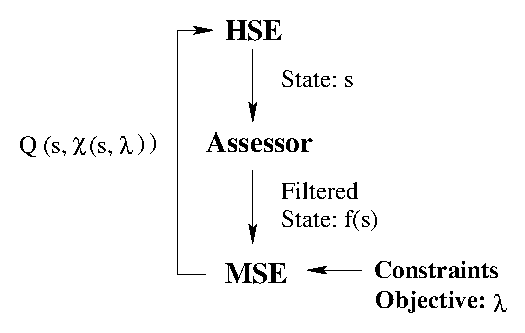
\includegraphics[scale=.75]{Graphics/rsmSchematic.eps}
 \end{center}
 \caption{\label{fig:rsmSchematic}  RSM schematic}
\end{figure}
 
\subsubsection{Linear Model}

HSE facilitates estimation of the hydrological states through a
linearized diffusion flow formulation. Typically, a linear model is
represented as a superposition of weighted states and forcing (or
basis) functions:
\begin{align}\label{eqn:linearModel}
  s(n) = \sum_{i=1}^{N}a_is(n-i) + \sum_{j=1}^Mb_j\Phi(n-j)
\end{align}

where $a_i$ and $b_j$ are model coefficients and $\Phi$ represent the
forcing terms. The task is then one of judiciously selecting the
coefficients to conform the model results to the observations. In HSE
[SFWMD1, 2005], the hydrologic representation is

\begin{align}\label{eqn:hseHydroRep}
 \mathbf{A}(\mathbf{H}) \cdot \frac{d\mathbf{H}}{dt} = \mathbf{q}(\mathbf{H}) + \mathbf{S}(\mathbf{H})
\end{align}

where $\mathbf{H}$ is a vector of finite volume waterbody states,
$\mathbf{q(H)}$ is a vector containing the summation of flow entering
the waterbodies, $\mathbf{S(H)}$ are non-gradient driven fluxes (source
terms) and $\mathbf{A(H)}$ is a diagonal matrix whose elements contain
the effective areas of the waterbodies. The flows $\mathbf{q(H)}$ are
linearized through use of a global flow resistance matrix
$\mathbf{M(H)}$:

\begin{align}\label{eqn:flowMatrix}
 \mathbf{q}(\mathbf{H}) = \mathbf{M}(\mathbf{H}) \cdot \mathbf{H}
\end{align}

The flows of equation \ref{eqn:flowMatrix} are solved with a PETSC
sparse linear system solver [SFWMD1 2005]. Once a solution of the
hydrologic states is available, dynamic evolution of the simulation is
specified as

\begin{align}
  s(n+1) = s(n) + \mathbf{A_n} \cdot \Delta \mathbf{H}
\end{align}

which is a special case of equation \ref{eqn:linearModel}. 

While many of the linearizations are well characterized, it is
possible that state variable regimes which invalidate the linear
assumptions could precipitate unanticipated model behaviors. The
chosen spatiotemporal discretizations of the model representation are
also capable of introducing nonlinear simulation artifacts. In
addition, there are likely nonlinear system variables which are
ignored by the model equations. Further, there may be inherent
limitations in the exclusion of hydrodynamic momentum terms from the
model formulation wherein stream flow dynamics are approximated. It is
known that the hydrological states are expressions of the dynamic
evolution of a nonlinear, chaotic timeseries [Park 2005], however, the
significant dissipation inherent in the physical system allows
reasonable approximations given well behaved linearizations ($ds/dt\ 
\alpha\ t$) and small enough simulation timesteps ($\Delta t \to$ 0).

\chapter{WMM Assessor}

The Water Management Model (WMM) Assessor refers to a combined state
variable assessor and interbasin water flow supervisor. It is based on
methodology implemented in the South Florida Water Management Model
(SFWMM)[SFWMD, 1999]\nocite{sfwmm:99}, and on code from the WCU
Assessors. The WMM Assessor estimates controlled basin structural
outflows to satisfy both water supply and flood control operational
constraints.

The WMM Assessor is designed to estimate the cumulative flows $Q_{nm}$
over a simulation timestep of one day. Currently, this is done through
an iterative procedure which updates state information from the HSE
for refined flow estimates in the WMM Assessor. This section documents
the WMM Assessor that is implemented for the SFRSM project.

\section{Assess Flow Function}\label{assessFunction}

The WMM Assessor interface in the RSM is contained in the Assess()
function. A flowchart schematic representation of this function is
shown in Figure \ref{fig:flowchartWMM}

\begin{figure}
 \begin{center}
  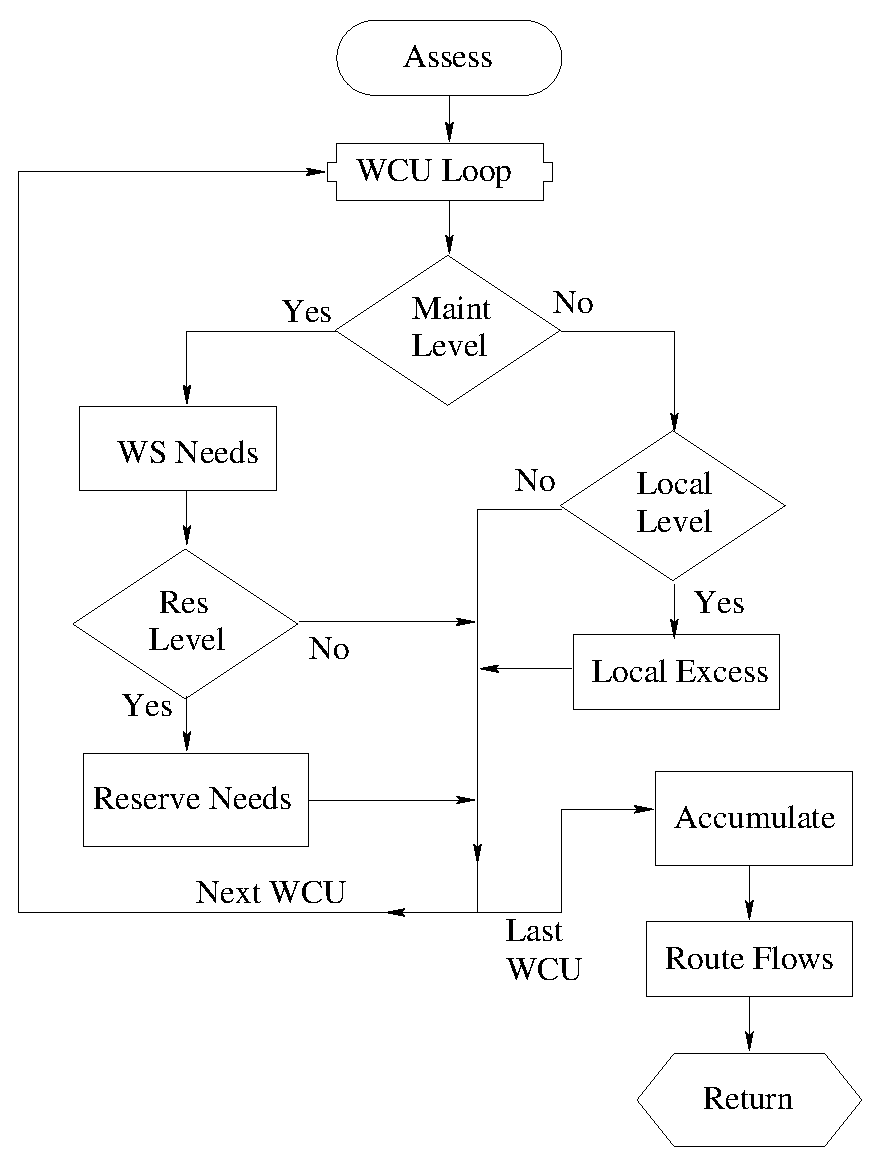
\includegraphics[scale=.33]{Graphics/flowchartWMM.eps}
 \end{center}
 \caption{\label{fig:flowchartWMM} Flowchart of WMM Assessor main
   function; Assess()}
\end{figure}

The Assess() function is executed before each solution of the HSE
state equations. Once the WCU outlet flows ($Q_{nm}$) are estimated,
these flows are imposed as boundary conditions on the HSE
solution. The Assess() function has three primary operations:

\begin{enumerate}
 \item Assess the volumetric supply or demand (needs) of each WCU 
 \item Accumulate the WCU needs across multiple, interconnected WCUs 
 \item Route WCU outlet flows to satisfy water supply needs and flood
   control objectives
\end{enumerate}

The water supply needs are evaluated by the three functions WSNeeds(),
ReserveNeeds() and LocalExcess(). These three functions perform
essentially the same computation: estimate the volume of water needed
to raise or lower a WCU to a target level, but with respect to three
different target water levels: MaintLevel, ResLevel and LocalLevel
respectively. The function which computes the water supply needs for
each target is the TargetVolume() function.

WSNeeds() is the volume of water required to bring the downstream end
of a WCU to its maintenance level. ReserveNeeds() is a smaller volume
than WSNeeds() and is the volume that will be supplied to a WCU if
water availability from upstream sources is limited. LocalExcess() is
the volume that a flow-thru WCU can provide as local water supply to
downstream WCUs. If a flow-thru WCU has excess volume, LocalExcess()
will return a negative volume.

\section {TargetVolume() function}

The primary computation of the TargetVolume() function is an estimate
of the total volumetric water differential needed to raise or lower
the water level of a WCU to satisfy a target water level. This
computation is specific to water supply needs or excesses, flood
control releases are computed separately in the RouteFlow() function.

Figure \ref{fig:WCUvolumeTarget} indicates a cross-sectional view of a
WCU consisting of four HSE canal segments. The water level difference
between the initial level and the target level at the downstream
control point is denoted $\Delta HT$. Once this target differential is
computed, it is added as an offset to each canal segment water level
in the WCU. These \emph{adjusted} water levels constitute a WCU water
level profile which defines the target water levels over the entire
WCU.

\begin{figure}
 \begin{center}
  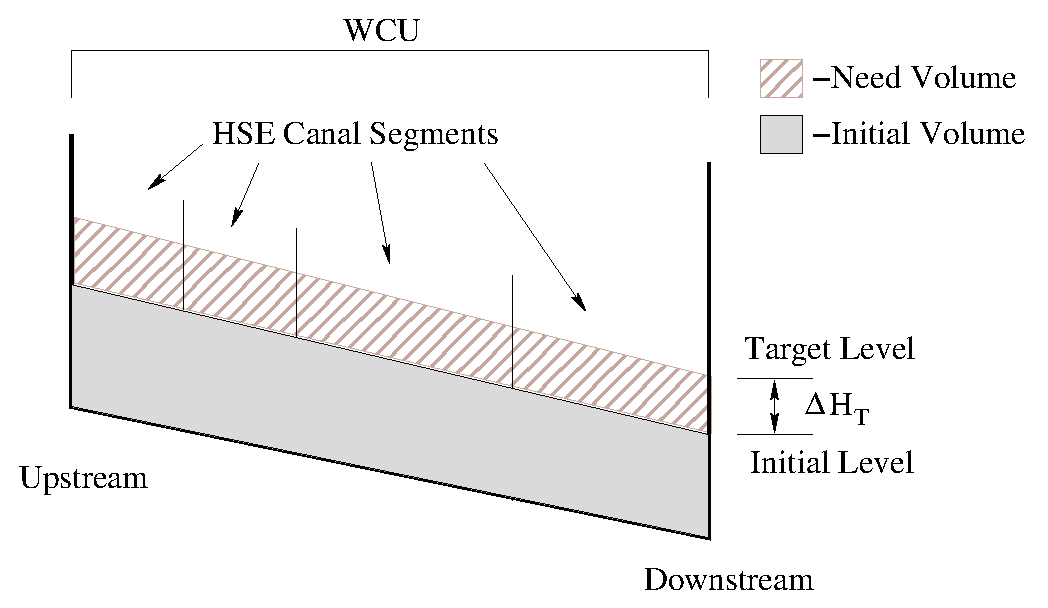
\includegraphics[scale=.5]{Graphics/WCUvolumeTarget.eps}
 \end{center}
 \caption{\label{fig:WCUvolumeTarget} WCU volume and target level for
   water supply needs}
\end{figure}

In the first HSE iteration, it is assumed that the target profile is
parallel to the previous time step profile. However, in subsequent
iterations, the target profile is assumed parallel to the profile
obtained in the previous sub-timestep iteration. 

Once the adjusted target profile is available, each canal segment in
the WCU is processed to estimate:

\begin{enumerate}
 \item Volume required to raise/lower the initial level to the target:
   $V_{H_t}$
 \item Canal segment water stage: $s_s(n) = s_s(n - 1) + \alpha_h \Delta H$ 
 \item Aquifer cell water stage: $s_c(n) = s_c(n - 1) + \alpha_h\Delta H$ 
 \item Volume of canal/aquifer seepage: $V_{SP} = f(s_s(n), s_c(n))$ 
 \item Volume canal overbank flow: $V_{OB} = f(s_s(n), s_c(n))$ 
 \item Volume of levee seepage: $V_{LV} = f(s_s(n), s_c(n))$ 
 \item Volume of boundary condition flows: $V_{BC}$ 
 \item Volume of WCU unmanaged (passive) structure inlets: $V_I (s_s(n))$ 
 \item Volume of WCU unmanaged (passive) structure outlets: $V_O(s_s(n))$
\end{enumerate}
 
where $s_s$ is the canal segment water level, $s_c$ the aquifer cell
water level, $a_h$ an implicit/explicit numerical solution weight
(SFWMDb, 2005)\nocite{sfwmdb:2005}, and $\Delta H$ the previous HSE
solution of state change. Boundary condition flows include HSE
watermovers defined by HSE boundary conditions, for example, a canal
segment may have a water stage boundary condition, or flow boundary
condition defined by a timeseries (SFWMDb,
2005)\nocite{sfwmdb:2005}. These estimates are then accumulated into a
final value of volumetric water supply need (WSN) for the WCU:

\begin{align} \label{eqn:wsn}
  V_{WSN} = \sum_{i=1}^{N} (V_{H_{T_i}} + V_{SP_i} + V_{OB_i} + V_{LV_i} + V_{BC_i} + V_{I_i} + V_{O_i})
\end{align}

where $N$ is the total number of canal segments in the WCU. The value
of $V_{WSN}$ is contained within the domain of $\Re$. Positive
$V_{WSN}$ indicates the deficit volume which needs to be added to the
WCU to meet the target level, negative $V_{WSN}$ signifies a volume of
excess water above the target level. The estimates of $V_{WSN}$ are
stored in data objects of each respective WCU for subsequent
reference.

\section {Accumulate() function}

After each WCU has been evaluated for water supply needs, the
Accumulate() function processes the entire WCU network to estimate the
cumulative water supply need at each WCU inlet. Figure
\ref{fig:flowchartAccumulate} depicts a schematic flowchart of the
Accumulate() function.

\begin{figure}
 \begin{center}
  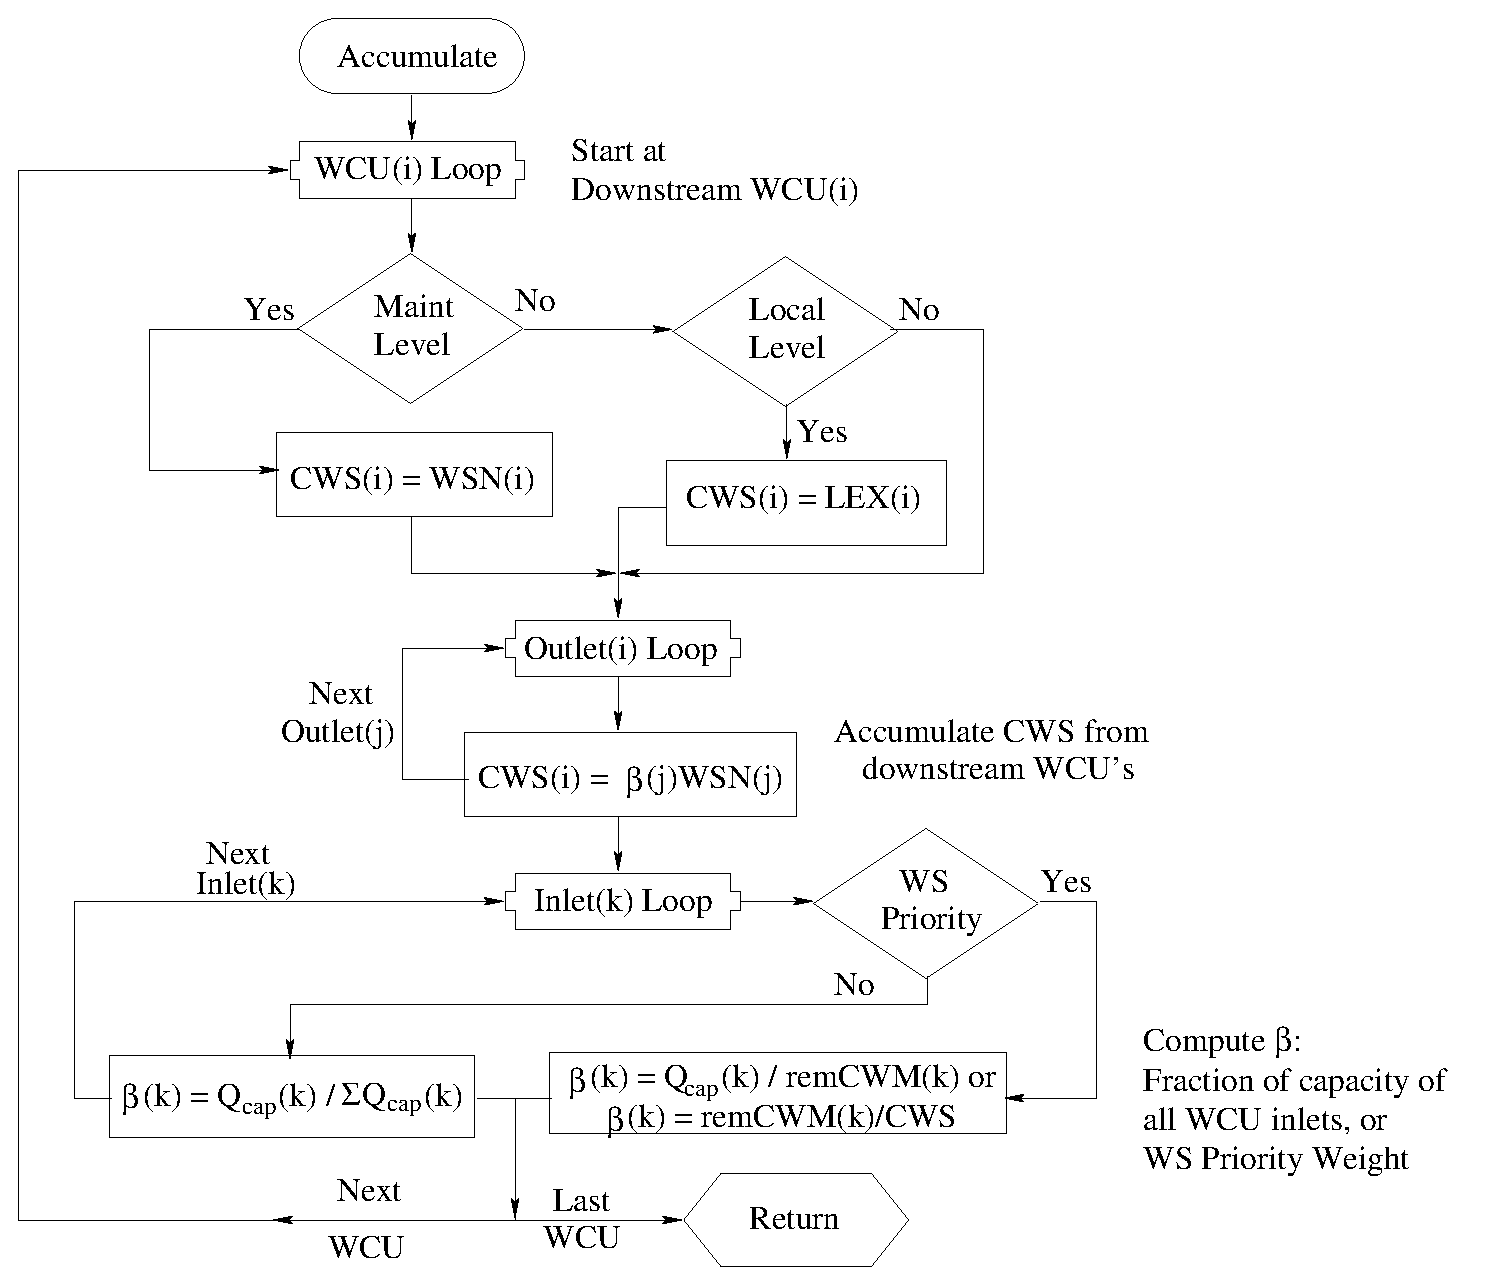
\includegraphics[scale=.33]{Graphics/flowchartAccumulate.eps}
 \end{center}
 \caption{\label{fig:flowchartAccumulate} Flowchart of WMM Assessor function; Accumulate()}
\end{figure}

The Accumulate() function contains three internal loops: 
\begin{enumerate}
 \item Process all WCUs from downstream to upstream (index(i)) 
 \item Process all outlets of a WCU to accumulate the CWS (index(j)) 
 \item Process all inlets of a WCU to compute capacity weight $\beta$
   (index(k)), or to set the water supply priority fraction of CWS for
   each inlet.
\end{enumerate}

The first (outer) loop ensures that all WCUs in the flow control
network are processed. The order of processing is determined by the
structure of the MSE Network definition file (SFWMDc,
2005)\nocite{sfwmdc:2005}. The first step in this loop is to
initialize the cumulative water supply need (CWS) for each WCU as
either the water supply need (WSN, positive or negative) or local
excess (LEX, negative) volume which were previously computed for each
WCU according to equation \ref{eqn:wsn} (see Figure
\ref{fig:flowchartWMM}).

The second loop then accesses all water supply outlet structures of
the current WCU, and accumulates their downstream CWS with the current
WCU. This accumulation is weighted by the flow capacity of the
downstream outlet structures. CWSj is limited to being greater than or
equal to 0, since excess water cannot be transferred upstream. The
third loop computes the a structure flow weight $\beta$ for all water
supply inlets of the current WCU. Since the processing of WCUs is from
downstream to upstream, a value of $\beta$ is always available for WCU
outlets in the second loop. $\beta$ is used for WCUs with multiple
water supply inlets to assign fractions of CWS to be met through
different routes. Computation of ß can be done in one of two modes. In
the default mode, the assumption is that routes with more capacity
will be used proportionally more for water supply, and therefore the
value of $\beta$ is simply a fraction of total WCU inlet capacity for
each inlet. Alternatively, if the WSPriority option is specified, then
each inlet is assigned an integer WSPriority value, lower integers
have higher priority. In this case, $\beta$ is computed to accommodate
available WS capacity for each inlet in order of priority, until the
WCU CWS needs are met.

\section {RouteFlow() function}

The functions described previously all fall under the functional
classification of assessors, they perform data filtering and
processing of state information to facilitate a decision
process. RouteFlow performs assessment functions, however it also
performs supervisory functions: it makes decisions on operational
flows imposed at flow control structures. A schematic flowchart of the
RouteFlow function is presented in Figure \ref{fig:flowchartRouteFlow}.

\begin{figure}
 \begin{center}
  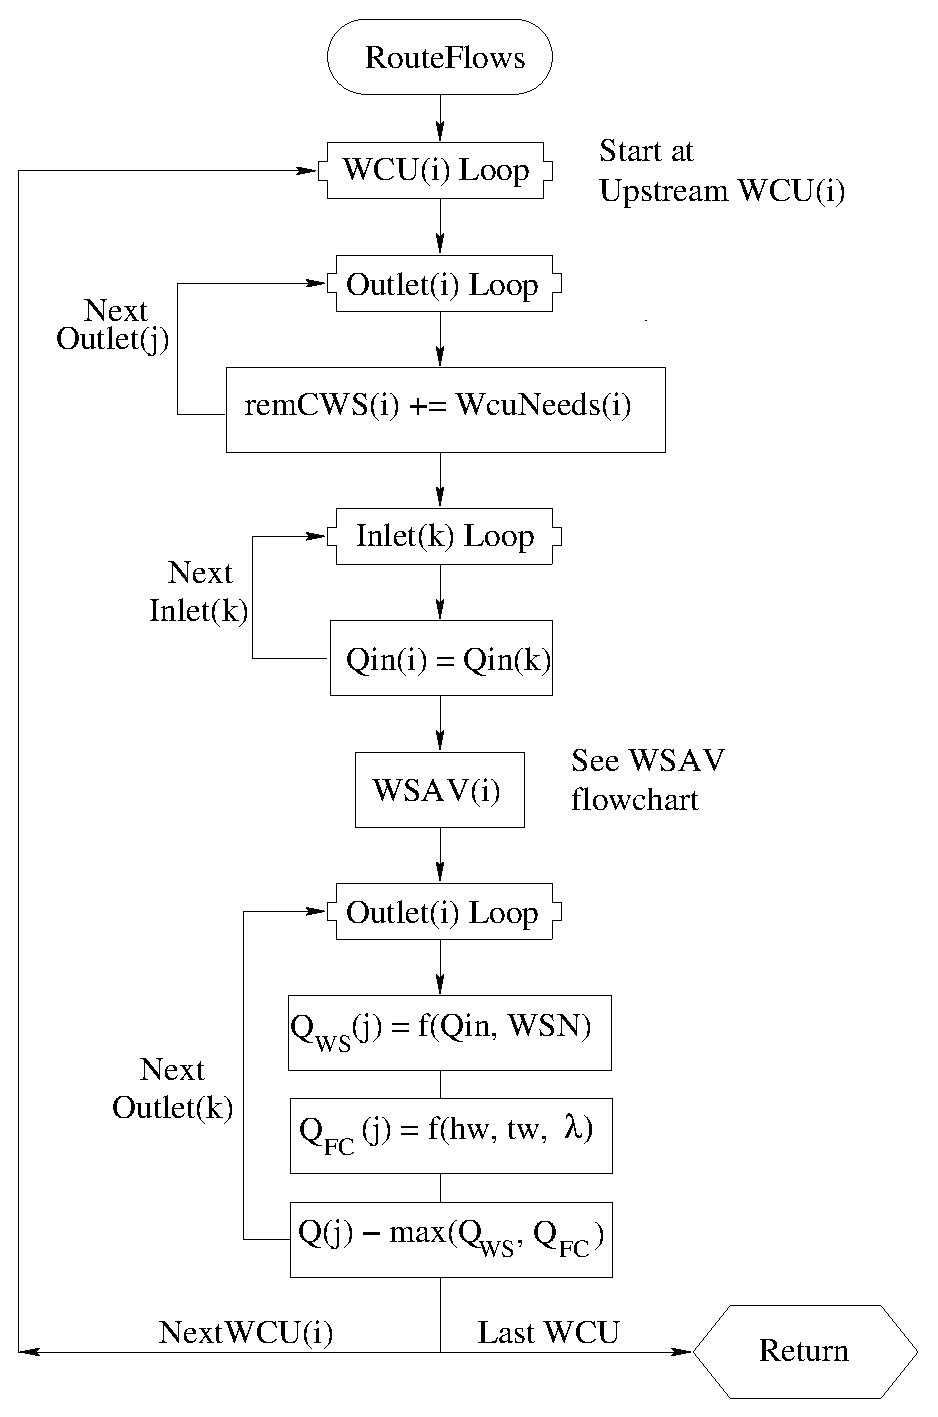
\includegraphics[scale=.33]{Graphics/flowchartRouteFlow.eps}
 \end{center}
 \caption{\label{fig:flowchartRouteFlow} Flowchart of WMM Assessor function: RouteFlow()}
\end{figure}
 
RouteFlow has a main (outer) loop which processes all WCUs starting at
the most upstream point, and sequentially progressing to the most
downstreamWCU as defined in the MSE Network definition file (SFWMDc,
2005)\nocite{sfwmdc:2005}. Since there is no recursive processing
involved, RouteFlow is not capable of balancing needs and flows that
change as a result of the flow decisions made in the single-pass
linear processing of WCUs. One of the ways in which this issue is
currently addressed is through the use of HSE-MSE iterations.

The following descriptions are with respect to a single WCU. The first
assessment in RouteFlow computes the remaining cumulative water supply
needs ($remCWS_i$) of the current WCU based on WCU outlets that are
designated as being Water Supply control structures. The computation
for a WCU with index $i$ that has water supply outlets with index $j$
is:

\begin{align}
  remCWS_i = \sum_j^N \beta _j CWS_j
\end{align}

Once the cumulative downstream needs have been compiled, the water
supply needs (WSN) for the WCU is computed by adding the local WCU WSN
to the $remCWS$:

\begin{align}
  CWS_i = WSN_L + remCWS_i
\end{align}

where $WSN_L$ represents the local WSN computed in Assess(). 

The next assessment to accumulate the total inflow from WCU inlet
structures, these individual values were computed previously for the
WCUs immediately upstream of the current WCU:

\begin{align}
  Q_{in_i} = \sum_j^N Q_k
\end{align}


Followed by a conditional assessment of the water supply available
volume (WSAV) based on cumulative structural inflows. $Q_{in_i}$  is converted to
a water supply available volume ($WSAV_i$) as follows:

\begin{align}
  WSAV_i = Q_{in_i} \Delta t
\end{align}

A schematic flowchart of $WSAV_i$ computation is shown in Figure
\ref{fig:flowchartWSAV}. Figure \ref{fig:flowchartWSAV} shows how
$WSAV_i$ is decremented as portions of it are assigned to the current
WCU and to downstream WCUs. These assignments depend on the purpose of
the current WCU and the magnitude of WSAV compared to needs.

\begin{figure}
 \begin{center}
  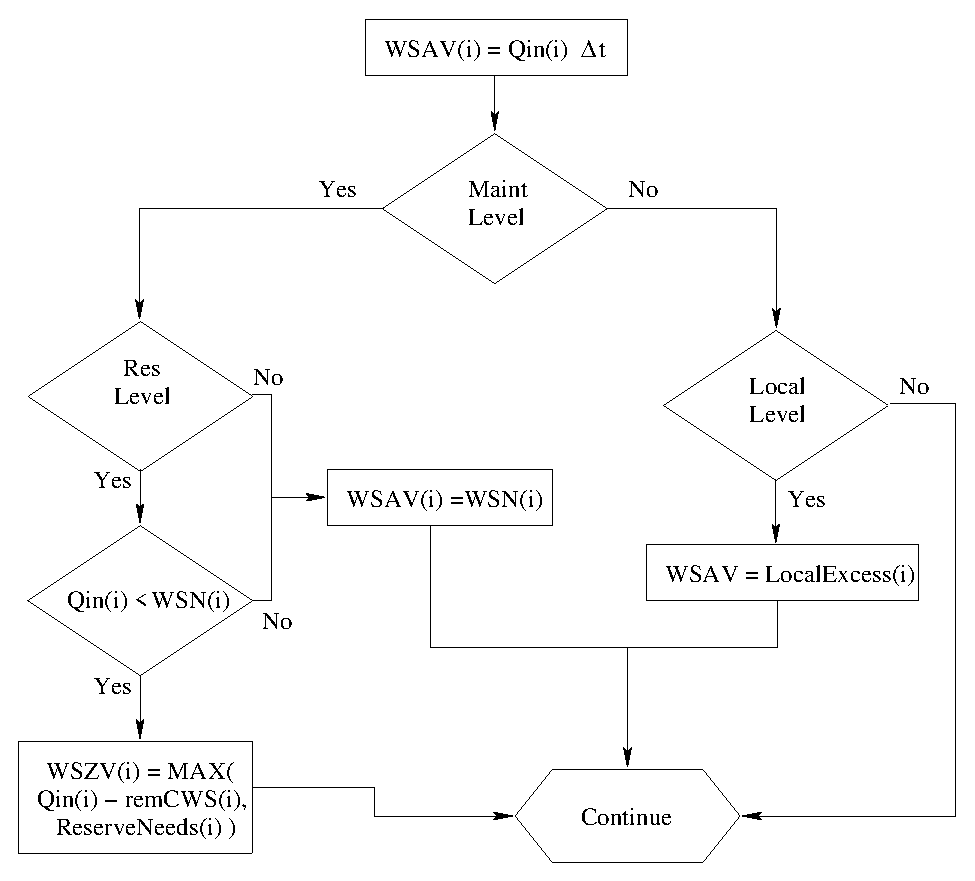
\includegraphics[scale=.33]{Graphics/flowchartWSAV.eps}
 \end{center}
 \caption{\label{fig:flowchartWSAV} Flowchart of Water Supply Available Volume (WSAV) in RouteFlow() function}
\end{figure}

If the currentWCU has a maintenance level but no reserve level, then
the first priority is to meet needs in the current WCU. Any remaining
portion of $WSAV_i$ will be available to meet needs in downstream
WCUs. If the current WCU has a maintenance level and a reserve level,
and there is not enough water available to meet all needs (i.e.,
$WSAV_i < CWS_i$), then only a portion of this WCU's needs are
met. The portion corresponds to at least the reserve level volume if
available. The remaining portion of $WSAV_i$ is available for
downstream WCUs. If the current WCU has local excess, it is added to
the available volume from upstream (i.e., a negative value is
subtracted from $WSAV_i$). For flow-through WCUs, all of $WSAV_i$ will
be available to meet needs in downstream WCUs.

Accordingly, WSAV can be expressed as: 
\begin{align}
 WSAV_i = \left\{
  \begin{array}{l l}
    Q_{in_i} \Delta t; & \quad initialvalue \\
    WSAV_i - MIN(WSAV_i, MAX(Q_{in_i}\Delta t - remCWS_i, ResNeeds_i)); & \quad ResLevel \\
    WSAV_i - WSN_i &\quad MaintLevel \\
    WSAV_i - LEX_i; & \quad LocalLevel \\
  \end{array} \right.
\end{align}


where LEX represents the Local Excess (negative) volume computed by LocalExcess(). 

\section{WS Flow Computation}
At this point in the RouteFlow() function the accumulated assessments
are completed, the processing now shifts to a supervisory mode wherein
the outlet flows are computed for each outlet of the respective WCUs.

The water supply (WS) flow for each water supply outlet structure is
based on the available volume of water in the WCU that can be used to
meet the cumulative downstream water supply needs. For each WS outlet
of the WCU, the available volume (AV) is computed according to a
shared adversity assumption:
\begin{align}
  AV_J &= (WSAV_j / remCWS) \cdot \beta_j &remCWS &> 0
\end{align}

where $CWS_j$ is the cumulative water supply need downstream of the
outlet.

The outlet WS flow for the structure with index j is specified as: 
\begin{align}
 Q_{WS_j} = MIN ( Q(hw, tw), AV_j / \Delta t)
\end{align}

where Q(hw, tw) is the current state flow capacity reported by the HSE
watermover. Note that hw and tw are the latest state estimates from
the previous HSE solution, these values may be from sub-timestep
iterations. The value of $Q_{WS}$ is then limited by the design
capacity of the structure.

The final step of the WS computation is to decrement the remCWS: 
\begin{align}
  remCWS_i \text{ -= } CWS_j \cdot \beta_j
\end{align}

and to decrement the WSAV of the WCU: 

\begin{align}
  WSAV_i \text{ -= } Q_{ws_j} \cdot \Delta t
\end{align}

\section{FC Flow Computation}

Flood control (FC) flows are based on water levels with respect to the
flood control criteria specified for each WCU outlet structure. The
criteria are expressed as an open and close water level. The FC flow
is:

\begin{align}\label{eqn:FCflow}
  Q_{FC_j} = \gamma_j \cdot Q_j(hw, tw)
\end{align}

where $\gamma$ represents a fractional value of total flow. $\gamma$
is based on a fractional gate opening for the structure fracGO:

\begin{align}
  fracGO = \frac {hw - close}{open - close}
\end{align}

 is computed as a power function (SFWMD, 1999).\nocite{sfwmm:99} 

\begin{align}
  \gamma = fracGO^b
\end{align}

where $b$ is a parameter usually set to 2. The resultant value of $Q_{FC}$
is limited by the design flow capacity of the outlet structure.

\section{Flow Assignment}
Once estimates for the WCU outlet water supply and flood control flows
are available, the final outlet flow value is simply a maximum of the
two values:
\begin{align}
  Q_j = MAX(Q_{WS_j}, Q_{FC_j})
\end{align}

This value is imposed as a boundary condition on the HSE solution of
Equation \ref{eqn:flowMatrix} for the structure watermover between the
respective WCU canal segments.

\section{MSE - HSE Convergence}\label{InfoMismatch}
A distinguishing feature of the HSE is the fully integrated
aquifer-stream flow solution. The finite volume hydrological
formulation expressed in Equation \ref{eqn:hseHydroRep} is solved in
one step (Equation \ref{eqn:flowMatrix}) for all waterbodies in the
model, inclusive of canal segments and aquifer cells. The HSE solution
is therefore an integrated global solution of the simulation
hydrologic processes. This feature is desirable from a physical
modeling perspective, as the physical system reacts as a global,
unitary, fully coupled system.

However, it is problematic from the point of view of MSE which
computes watermover flows independently of the conjunctive HSE
solution. The essential difficulty is that the MSE decisions are based
on previous HSE solution state information, but are imposed on the
next HSE solution as flow boundary conditions. As the simulation
timestep duration increases ($\Delta t = t_e - t_s$ of Equation
\ref{eqn:CumBasintoBasin} becomes large) the divergence between the
actual cumulative flow $Q_{mn}$, and the flow estimated by the WMM Assessor
$Q_{mn}$ increases. This divergence arises for several reasons:

\begin{enumerate}
  \item $Q_{mn}$ is based on previous timestep state information. 

  \item Nonlinearities approximated in the global HSE solution of the
    equations are not modeled in the WMM Assessor.

  \item Lack of synoptic (multipleWCU) balancing of headwater and
    tailwater in the WMM Assessor.
\end{enumerate}

An observational result of this divergence is the WCU Profile Mismatch
which precipitates canal stage \emph{oscillations}. 

\section{WCU Profile Mismatch}
Consider a coupled set of upstream-downstream WCUs with a single
controlled flow structure between WCUs as illustrated in Figure
\ref{fig:wcusCoupled}. Each WCU has MSE controlled structural inflow
and outflow, for example structure $S_{01}$ controls flow $Q_{01}$
into $WCU_1$, and structure $S_{12}$ controls flow $Q_{12}$ out of
$WCU_1$ into $WCU_2$. These cumulative structural flows are estimated
by the WMM Assessor. Each WCU is also subjected to boundary
condition and hydrologic state influenced inflows and outflows ($Q_s$)
which include aquifer-canal seepage, rainfall, and all other
non-structural fluxes. Operational criteria for a WCU can include a
water supply maintenance level $T_{WS}$, and flood control level
$T_{FC}$ specified at the downstream end of a WCU.

 \begin{figure}
 \begin{center}
  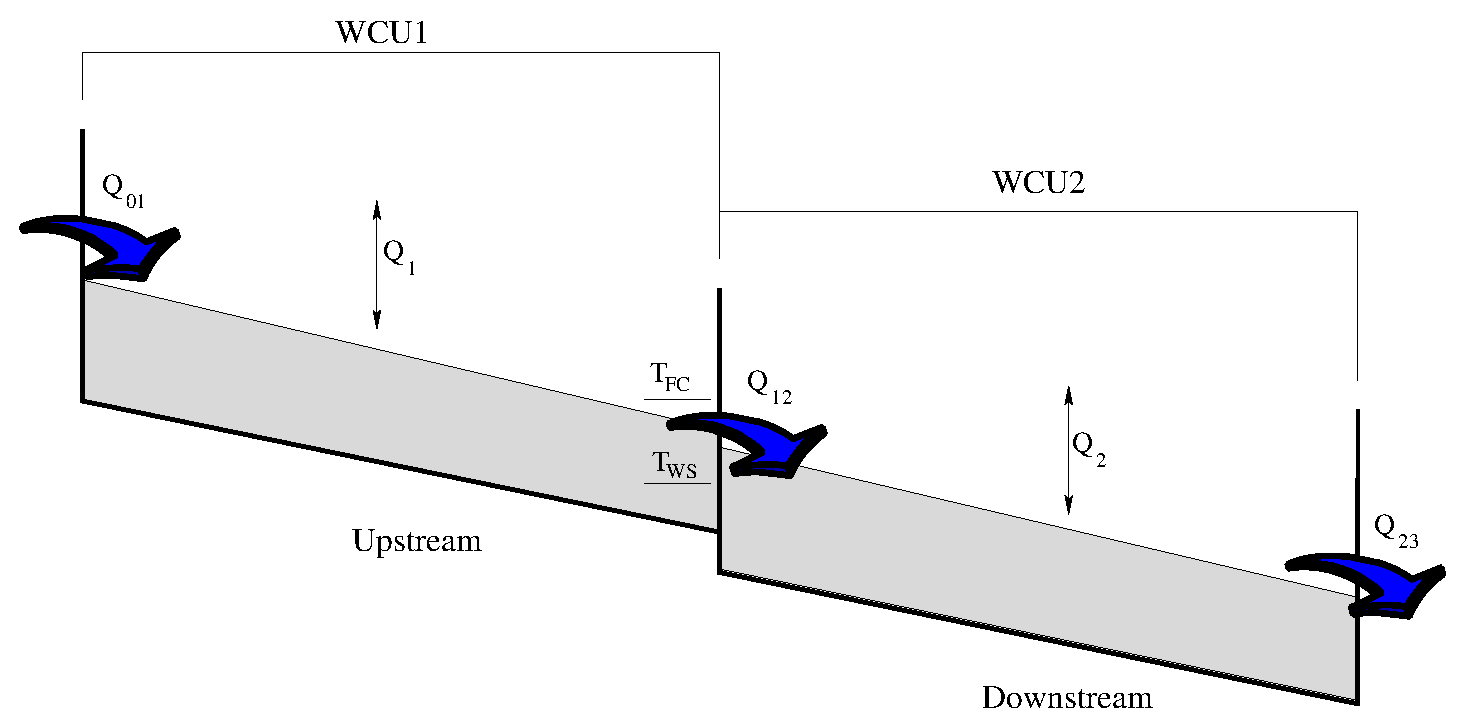
\includegraphics[scale=.33]{Graphics/wcusCoupled.eps}
 \end{center}
 \caption{\label{fig:wcusCoupled} Two WCUs coupled by a structure with flow $Q_{12}$}
\end{figure}

Interbasin flow estimates for the next timestep ($Q_{12}(n + 1)$) are
based on previous timestep information ($s(n),Q_s(n)$) and are likely
to differ from the actual flows $Q_{12}(n + 1)$. Further, these
estimates are imposed as flow boundary conditions on Equation
\ref{eqn:flowMatrix} for the next timestep (n+1) solution. The
imposition of an erroneous estimate can produce significant impacts on
the global hydrologic solution. In the case of a positive residual
$\Delta Q_{12} = Q_{12} - Q_{12} > 0$; where the estimated flow is
less than the ideal flow, the upstream WCU will contain excess water
and will result in a $WCU_1$ water level profile that is higher than
that \emph{expected} by the ideal solution. The deficit of transfer
flow from $WCU_1$ to $WCU_2$ will also result in a lower water level
in $WCU_2$ than would occur with the correct flow value. This
situation is depicted in Figure \ref{fig:wcusCoupled_1}.

 \begin{figure}
 \begin{center}
  \includegraphics[scale=.33]{Graphics/wcusCoupled_1.eps}
 \end{center}
 \caption{\label{fig:wcusCoupled_1} WCU state if estimated flow $Q_{12}$ is less than actual $Q_{12}$.}
\end{figure}

As a result of the positive flow residual, the headwater of structure
$S_{12}$ is above that of the correct value while the tailwater is
below the expected value. This increased head differential will
produce a larger potential structure flow (the flow produced by
application of the structure watermover transfer function to the
applied headwater and tailwater) than the correct value. These
erroneous water levels and the incorrect potential flow will be used
in the next timestep. Another issue concerns the flood control target
level of $WCU_1$. The estimated WCU water level exceeds the flood
control level, while the correct value does not. The result would be
an incorrect flood control flow release for structure $S_{12}$.

Consider now a negative flow residual: $\Delta Q_{12} = Q_{12} -
Q_{12} < 0$; where the estimated flow is greater than the actual flow,
the resultant WCU water levels could be as shown in Figure \ref{fig:wcusCoupled_2}.

 \begin{figure}
 \begin{center}
  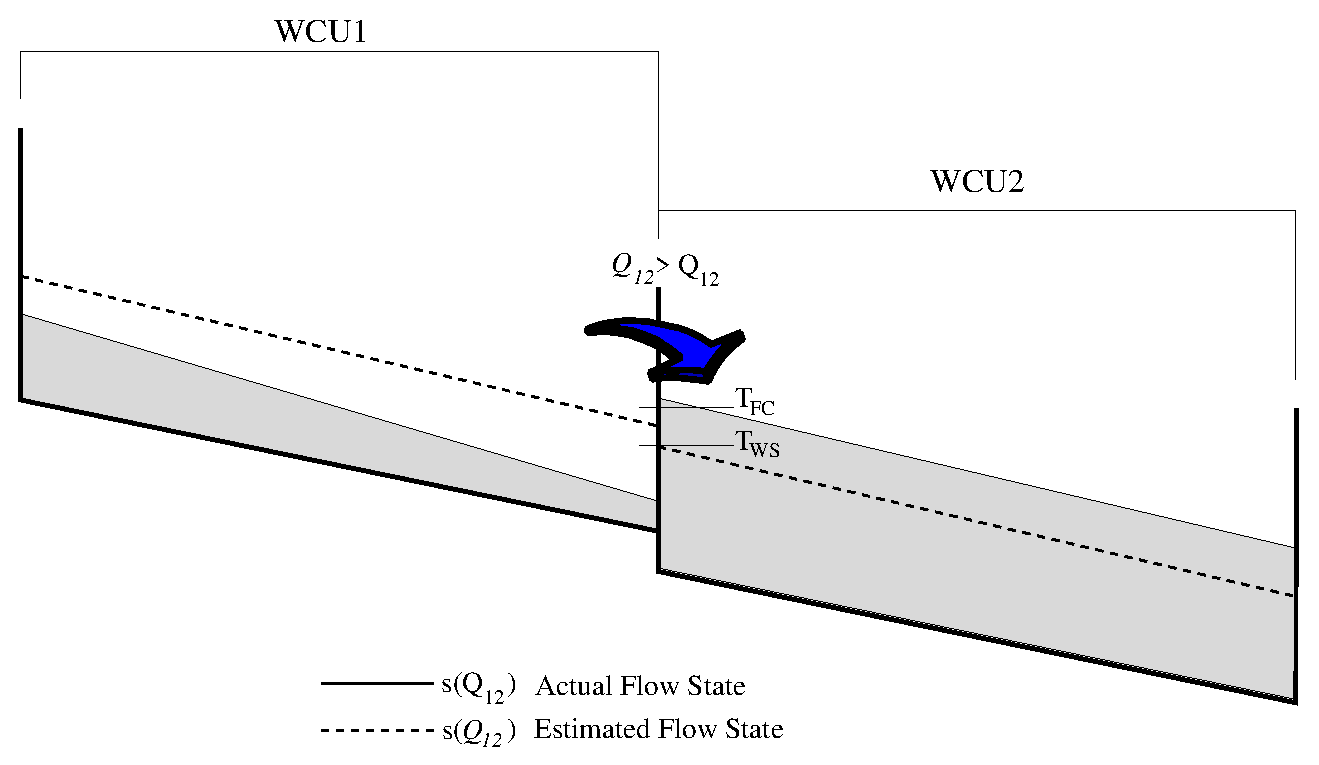
\includegraphics[scale=.33]{Graphics/wcusCoupled_2.eps}
 \end{center}
 \caption{\label{fig:wcusCoupled_2} WCU state if estimated flow $Q_{12}$ is greater than actual $Q_{12}$.}
\end{figure}

The negative flow residual has created a water level inversion, the
tailwater of structure $S_{12}$ is above the headwater. The potential
flow of the structure will be zero. The resultant water level in
$WCU_1$ can also fall below the water supply threshold, whereas the
actual value would not. The erroneous potential flow and threshold
crossing will result in incorrect flow computations on the next
timestep.

\section{MSE Induced Oscillation}
There are many causes of canal water level oscillations in hydraulic
numerical models, for example, improper spatiotemporal
discretizations, numerical threshold crossings, or uncompensated
control signals applied to hydraulic flows.

Consider the situation presented in Figure \ref{fig:wcusCoupled_1}
where the WMM Assessor encounters a water level in $WCU_1$ above the
flood control threshold $T_{FC}$. The reason for this water level,
whether through estimation inaccuracy or levels match the actual
values, is not germane. The WMM Assessor will compute a flood control
release flow according to Equation \ref{eqn:FCflow}. This value of
$Q_{12} = Q_{FC}$ will be relatively large with respect to the
structure flow capacity. The large flow can result in significant
reduction of water level in $WCU_1$ for the next timestep, lowering
the level below the flood control threshold analogous with Figure
\ref{fig:wcusCoupled_2}. After the next timestep the $WCU_1$ level may
be low enough that no flow release is warranted, thereby setting
$Q_{12} =0$. If the upstream structural and other inflows ($Q_{12} + Q_s$)
are significant enough, then in the following timestep the levels in
$WCU_1$ may again rise above $T_{FC}$, and the cycle repeats.

This cyclic recurrence of control limit states, $\Delta Q_{12} =
Q_{FC}; Q_{12} = 0$, is commonly referred to as \emph{bang-bang}
control, or \emph{slamming}. The controller is slamming between
maximal control points due to saturation of the control input state
variables. Typical solutions entail filtering of the input states,
and/or incorporation of an integration term in the control
algorithm. In the current WMM Assessor implementation, an alternative
approach is used where a convergence function is applied to limit the
changes in estimated interbasin flow ($Q_{mn}$) so that a global
solution can be found based on HSE state information feedback.

Even though slamming appears to the primary cause of observed canal
oscillations, and this limit cycle behavior is certainly dependent on
the nonzero flow estimate residuals, it is possible that the
inaccuracies and nonzero flow estimate residuals themselves can
produce oscillations as described in Section \ref{InfoMismatch}.

\section{MSE - HSE Iterations}
Recognizing that the WMM Assessor estimated flow residuals diverge as
the simulation timestep increases, a natural solution is to provide
iterative HSE state information updates in in order to refine the
estimated flows within a timestep. An error metric which quantifies
the flow estimate divergence is used to terminate the iterations when
a convergence threshold is satisfied. RSM performs this iterative flow
refinement in three basic steps:

\begin{enumerate}
  \item WMM Assessor estimates flows $Q_A$ based on the latest HSE
    iteration state information ($\Sigma (j-1)$) and management constraints
    ($\lambda$).

  \item Estimated flow ($Q_A$) changes are limited with a convergence
    function to produce the final estimated flow $Q$.

  \item New HSE state estimates are solved by imposition of the
    estimated flows $Q$ applied to previous timestep state conditions
    ($\Sigma (i)$).
\end{enumerate}

A schematic flowchart of the MSE - HSE iteration is shown in Figure
\ref{fig:flowchartIteration}. Referring to Figure
\ref{fig:flowchartIteration}, there are two processing loops
shown. The outer loop represents a HSE timestep and is indexed with
the variable $i$. As i changes from $i$ to $i+1$, the HSE simulation has
advanced forward by one timestep ($\Delta t$). The inner loop depicted in
Figure \ref{fig:flowchartIteration} is the MSE - HSE iteration loop,
it is represented with the iteration index $j$.

\begin{figure}
 \begin{center}
  \includegraphics[scale=.33]{Graphics/flowchartIteration.eps}
 \end{center}
 \caption{\label{fig:flowchartIteration} Schematic flowchart of
   HSE-MSE iteration algorithm.}
\end{figure}

The first computation estimates the desired flow QA based on the
latest state information which will satisfy the operational
constraints, thus:

\begin{align}
  Q_A = m [ \Sigma (j - i), \lambda ]
\end{align}

where m[] indicates the WMM Assessor processing described in Section
\ref{assessFunction}. The argument $\Sigma(j-1)$ refers to the HSE
state information obtained from the previous (latest) HSE iteration,
and as before $\lambda$ refers to the managerial constraints such as
WCU target levels for water supply and flood control. Therefore, the
first step consists of estimating the flows required to meet the
operational constraints where the state information is taken from the
HSE solution based on the most recent WMM Assessor flow estimates. It
is assumed that the most recent HSE state information allows better
quantification of WCU inflows and outflows than could easily be
obtained from the beginning of timestep state $\Sigma (i)$.

Experience with simulation of $Q_A$ has shown that oscillations of
assessed flow (and the corresponding water levels) are common, owing
to control point saturation and state variable inaccuracies (see
Section \ref{InfoMismatch}). The second primary computation implements
a straightforward, if somewhat inelegant solution to this problem by
imposition of a Markovian weighting to the estimated flow changes:

\begin{align} \label{eqn:convergenceFunction}
  Q(j) = c[Q_A(j),Q(j - 1),\alpha(j)] = \alpha(j)Q_A(j) + (1 - \alpha(j))Q(j - 1)
\end{align}
where $\alpha$ is a weighting factor in the domain $\Re \subset
[1,0]$. The convergence function $c[]$ provides values of a at each
iteration. One can view this limiting of flow change as consistent
with the significant dissipation inherent in the hydrologic dynamic
system, a requirement for a stable manifold of the chaotic dynamics.

Once the estimated, weighted flows are available, the third step is to
impose these flows on the HSE state from the previous timestep to
compute a current state estimate $\Sigma (j)$:

\begin{align}
  \Sigma (j) = h \left [ Q(i), \Sigma (i) \right ]
\end{align}

where h[] indicates solution of the HSE (Equation
\ref{eqn:flowMatrix}) based on the previous timestep state conditions
$\Sigma$ (i), and the WMM Assessor imposed flows $Q(j)$.

The final step is to decide whether or not the estimated flows and
resultant states are satisfactory; whether or not to continue the
iterations. This is done by comparing the global flow residuals
$\Delta Q = Q-Q$ to a user defined threshold $\epsilon$ , where the
desired flow value is the unweighted, assessed flow from the WMM
Assessor, in other words $Q = Q_A$ so that:

\begin{align}
  \Delta Q = Q_A - Q
\end{align}

This ensures that the final MSE imposed flows converge to the flows
which satisfy the operational constraints included in the computations
of the WMM Assessor. By basing the convergence criteria on a flow
threshold applied to residuals, the user can control a tradeoff
between accuracy of the final estimate and the number of
iterations. Another result is that the number of iterations is related
to the variability of the state conditions. In effect, one can
consider the MSE - HSE Iterations as a state dependent implementation
of variable timesteps. For example, in relation to the daily timestep
$\Delta t$ = 1 day = 1440 minutes; a terminal iteration at $j$=144
would correspond to the same computational overhead as a 1440/144 = 10
minute timestep.

It is important to note that the WMM Assessor makes flow estimates
based on state information from the previous iteration. As the flow
estimates improve and decrease the flow residuals, the accuracy of the
WCU inflows/outflows increases. However, at the end of each iteration,
the estimated flows are imposed on the previous timestep state
conditions. This ensures that the final flows are consistent with the
state evolution from the previous timestep to the next timestep.

\section {WMM Assessor Convergence Function}
The convergence function plays a critical role in allowing the WMM
Assessor to find a global solution for flows which are both consistent
with the HSE hydrological states, and satisfies the operational
constraints. Essentially, the convergence function expressed in
Equation \ref{eqn:convergenceFunction} limits the change in state of
the estimated flows from one iteration to the next. This is consistent
with the observed nature of the system dynamics wherein dissipation
(damping) is inherent. The \emph {degree of dissipation} is
encapsulated in the function $\alpha(j)$. Several different functions
for $\alpha$(j) were evaluated, and the current default function for
WMM Assessor is QDELTA\_MAX2.  It is essentially a moving hard-limiter
function. Instead of using a variable $\alpha (j)$ function to
constrain the flow changes, a threshold limit is applied at each
iteration. The threshold is specified with the maxQDelta XML attribute
of the WMM Assessor. At each iteration, if the change in flow from the
previous iteration is less than maxQDelta, then that value of flow is
assigned to the $Q(j)$. If the change in flow is greater than
$maxQDelta$, then the change in flow is limited to $maxQDelta$:

\begin{align}
  Q(j) = Q(j-1) \pm maxQDelta
\end{align}

